\section{Other Path Planning}
Probably going to end up removing this section, but the math in it led me to the math of the previous section. 

\subsection{One Dimensional Hazard}
Now assume that there is a hazardous area that has a relative cost proportional to the distance from the y axis, i.e. some value $f(x)$. Assuming zero cost elsewhere, the shortest path is going to be similar to the path shown in figure \ref{oneD}.
\begin{figure}
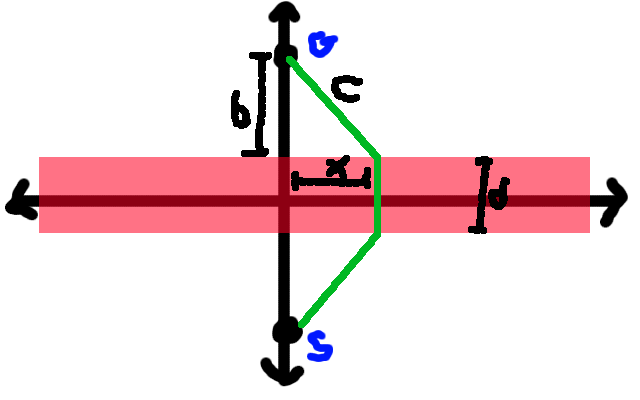
\includegraphics[width=\columnwidth]{graphix/oneD.png}
\label{oneD}
\caption{One Dimensional Setup}
\end{figure}
Let us define the path going through point $(x,0)$ to be $p(x)$. The cost of such a path will be 
\begin{align*}
C(p(x)) &= P * (2*c+d) + f(x) \\ 
 &= P * (2 * \sqrt{x^2 + b^2} + d) + f(x)
\end{align*}
If we want to force the path to cross at a certain point (call it $m$), we need to set $f(x)$ in such a way that $C(p(x))$ is a minimum. To do that we take the derivative of $C(p(x))$. 
\begin{align*}
C'(p(x)) &= f'(x) + \frac{2Px}{\sqrt{x^2+b^2}} \\
\intertext{If we set the derivative to 0}
f'(x) &= -\frac{2Px}{\sqrt{x^2+b^2}}
\intertext{Since we assert that this minimum occurs at $x=m$}
&= -\frac{2Pm}{\sqrt{m^2+b^2}}
\intertext{Integrating we get...}
f(x) &= D - \frac{2Pmx}{\sqrt{m^2+b^2}}
\end{align*}
for some constant D. 
